% thanks to Claude for the skeleton

\documentclass{standalone}
\usepackage{tikz}
\usetikzlibrary{calc}

\newcommand*{\LT}{u}
\newcommand*{\LB}{x}
\newcommand*{\RT}{y}
\newcommand*{\RB}{v}

\begin{document}
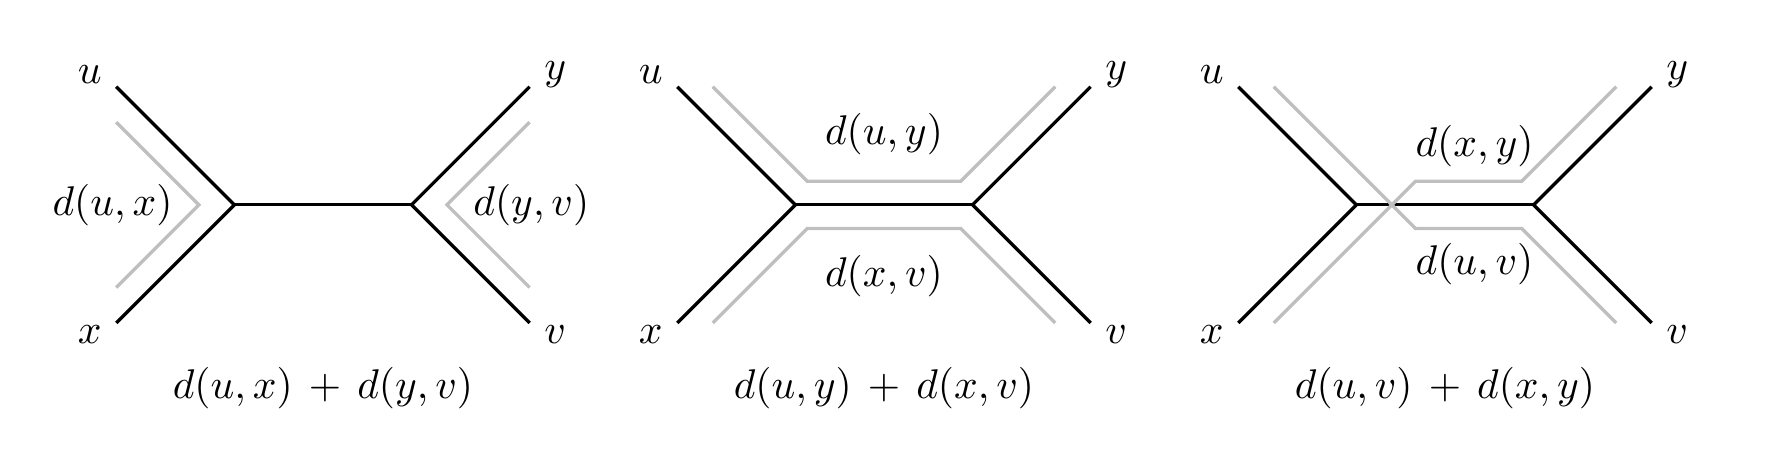
\begin{tikzpicture}[scale=1.5, every node/.style={scale=1.5}]

\useasboundingbox (-6.5,-2) rectangle (8,1.5);
% \draw[help lines] (-10,-10) grid (10,10); % grid
% \draw[ultra thick, ->] (-10,0) -- (10,0); % x-axis
% \draw[ultra thick, ->] (0,-10) -- (0,10); % y-axis
% \fill[red] (0,0) circle (0.1); % Red dot at the origin

% First diagram
\begin{scope}[xshift=-4.75cm]
    % Black lines
    \draw[black, very thick] (-1,1)  -- (0,0)   -- (-1,-1);
    \draw[black, very thick] (0,0)   -- (1.5,0);
    \draw[black, very thick] (2.5,1) -- (1.5,0) -- (2.5,-1);
    % Light gray lines
    \draw[lightgray, very thick] (-1,0.7)  -- (-0.3,0) -- (-1,-0.7);
    \draw[lightgray, very thick] (2.5,0.7) -- (1.8,0)  -- (2.5,-0.7);
    % Nodes labels
    \node[left]   at (-1,1.1)    {$\LT$};
    \node[left]   at (-1,-1.1)   {$\LB$};
    \node[right]  at (2.5,1.1)   {$\RT$};
    \node[right]  at (2.5,-1.1)  {$\RB$};
    % Edges labels
    \node[left]   at (-0.4,0)      {$d(\LT,\LB)$};
    \node[right]  at (1.9,0)       {$d(\RT,\RB)$};
    \node[below]  at (0.75,-1.25)  {$d(\LT,\LB) \,+\, d(\RT,\RB)$};
\end{scope}

% Second diagram
\begin{scope}
  % Black lines
    \draw[black, very thick] (-1,1)  -- (0,0)   -- (-1,-1);
    \draw[black, very thick] (0,0)   -- (1.5,0);
    \draw[black, very thick] (2.5,1) -- (1.5,0) -- (2.5,-1);
    % Light gray lines
    \draw[lightgray, very thick] (-0.7,1)  -- (0.1,0.2)  -- (1.4,0.2)  -- (2.2,1);
    \draw[lightgray, very thick] (-0.7,-1) -- (0.1,-0.2) -- (1.4,-0.2) -- (2.2,-1);
    % Nodes labels
    \node[left]   at (-1,1.1)    {$\LT$};
    \node[left]   at (-1,-1.1)   {$\LB$};
    \node[right]  at (2.5,1.1)   {$\RT$};
    \node[right]  at (2.5,-1.1)  {$\RB$};
    % Edges labels
    \node[above]  at (0.75,0.3)    {$d(\LT,\RT)$};
    \node[below]  at (0.75,-0.3)   {$d(\LB,\RB)$};
    \node[below]  at (0.75,-1.25)  {$d(\LT,\RT) \,+\, d(\LB,\RB)$};
\end{scope}

% Third diagram
\begin{scope}[xshift=4.75cm]
    % Black lines
    \draw[black, very thick] (-1,1)  -- (0,0)   -- (-1,-1);
    \draw[black, very thick] (0,0)   -- (1.5,0);
    \draw[black, very thick] (2.5,1) -- (1.5,0) -- (2.5,-1);
    % Light gray lines
    \draw[lightgray, very thick] (-0.7,1)  -- (0.5,-0.2) -- (1.4,-0.2) -- (2.2,-1);
    \draw[lightgray, very thick] (-0.7,-1) -- (0.5,0.2)  -- (1.4,0.2)  -- (2.2,1);
    % Nodes labels
    \node[left]   at (-1,1.1)    {$\LT$};
    \node[left]   at (-1,-1.1)   {$\LB$};
    \node[right]  at (2.5,1.1)   {$\RT$};
    \node[right]  at (2.5,-1.1)  {$\RB$};
    % Edges labels
    \node[above]  at (1,0.2)       {$d(\LB,\RT)$};
    \node[below]  at (1,-0.2)      {$d(\LT,\RB)$};
    \node[below]  at (0.75,-1.25)  {$d(\LT,\RB) \,+\, d(\LB,\RT)$};
\end{scope}

\end{tikzpicture}
\end{document}